\documentclass[border=6pt]{standalone}
% Shared typography and colours for the standalone figures.
\usepackage{unicode-math}
\setmainfont{TeX Gyre Heros}
\setmathfont{TeX Gyre Pagella Math}
\usepackage{tikz}
\usetikzlibrary{arrows.meta,positioning,calc,decorations.pathreplacing}
\usepackage{pgfplots}
\pgfplotsset{compat=1.18}

% One colour per element or subsystem. Record the mapping in
% the working repository conventions and use it identically in every figure.
\definecolor{elemA}{HTML}{1F5FA8}
\definecolor{elemB}{HTML}{B8461B}
\definecolor{elemC}{HTML}{2E7D32}
\definecolor{elemD}{HTML}{6A4C93}
\definecolor{frameline}{HTML}{555555}

\begin{document}
\hyphenpenalty=10000
\exhyphenpenalty=10000
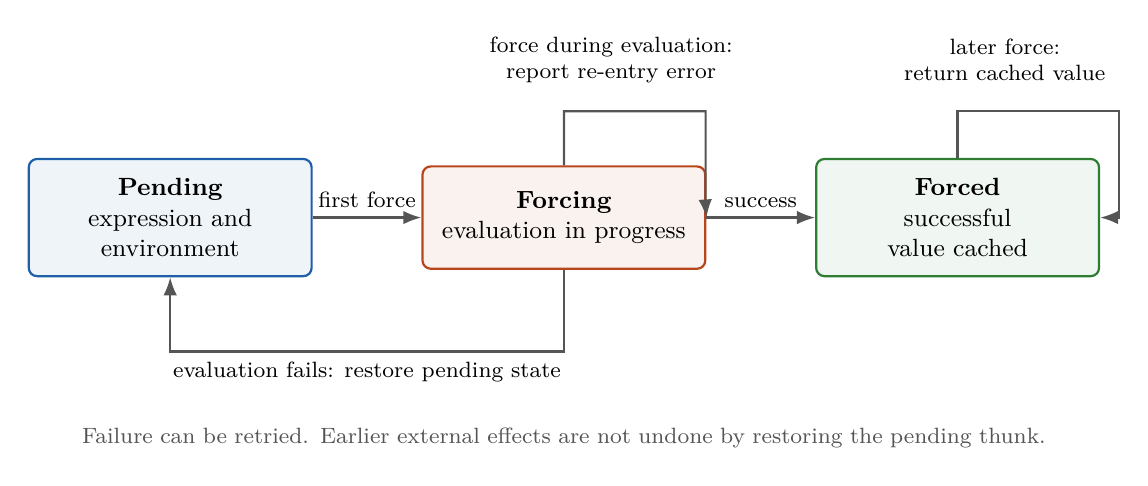
\begin{tikzpicture}[font=\small,
state/.style={draw=#1,fill=#1!7,rounded corners=3pt,line width=.8pt,text width=3.1cm,minimum height=1.3cm,align=center,inner sep=7pt},
arrow/.style={-{Latex[length=2.3mm]},line width=.8pt,draw=frameline}]
\node[state=elemA] (pending) at (-5,0) {\textbf{Pending}\\expression and environment};
\node[state=elemB] (forcing) at (0,0) {\textbf{Forcing}\\evaluation in progress};
\node[state=elemC] (forced) at (5,0) {\textbf{Forced}\\successful value cached};
\draw[arrow] (pending)--node[above,font=\footnotesize]{first force}(forcing);
\draw[arrow] (forcing)--node[above,font=\footnotesize]{success}(forced);
\draw[arrow] (forcing.south) -- (0,-1.7) --node[below,font=\footnotesize]{evaluation fails: restore pending state} (-5,-1.7)--(pending.south);
\draw[arrow] (forcing.north) -- (0,1.35) -- (1.8,1.35) -- (1.8,.15) -- (forcing.east);
\node[font=\footnotesize,align=center] at (.6,2) {force during evaluation:\\report re-entry error};
\draw[arrow] (forced.north) -- (5,1.35) -- (7.05,1.35) -- (7.05,0) -- (forced.east);
\node[font=\footnotesize,align=center] at (5.6,2) {later force:\\return cached value};
\node[font=\footnotesize,text=frameline,align=center,text width=12.5cm] at (0,-2.8)
 {Failure can be retried. Earlier external effects are not undone by restoring the pending thunk.};
\end{tikzpicture}
\end{document}
